% !TeX root = ../../Skript.tex
\cohead{\Large\textbf{Extrempunkte}}
\fakesubsection{Extrem- und Sattelpunkte}
\textbf{Hochpunkt}

Ein Hochpunkt hat den größten Funktionswert in seiner Umgebung.

\medskip

\begin{minipage}{\textwidth}
	\adjustbox{valign=t, padding = 0ex 0ex 2ex 0ex}{\begin{minipage}{\textwidth/\real{3}-2ex}
			\centering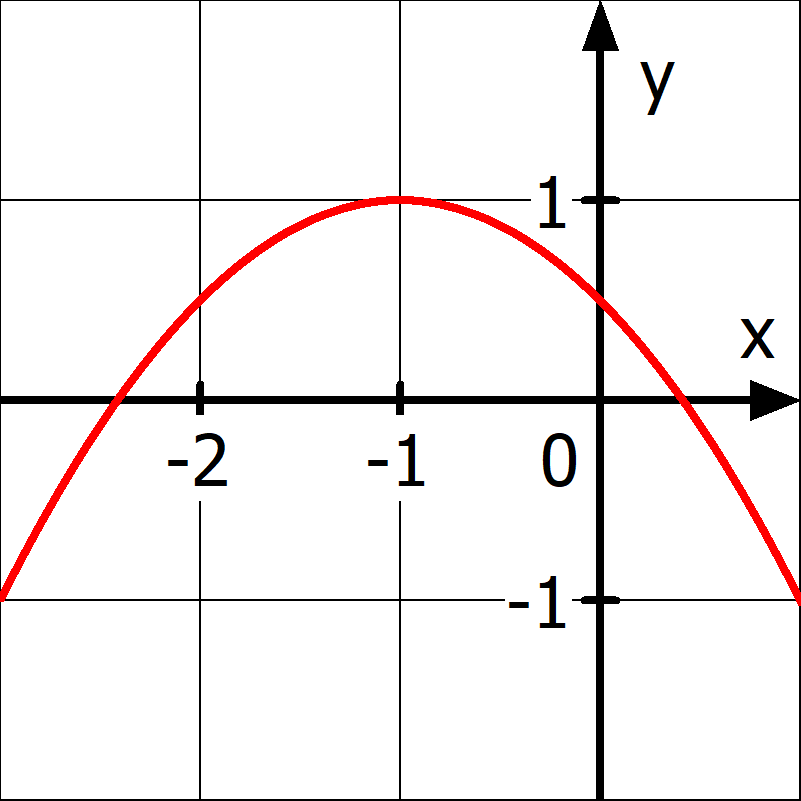
\includegraphics[width=\textwidth]{\ableitung/pics/HPBsp.png}
	\end{minipage}}%
	\adjustbox{valign=t, padding = 0ex 0ex 2ex 0ex}{\begin{minipage}{\textwidth/\real{3}-2ex}
			\centering\includegraphics[width=\textwidth]{\ableitung/pics/HPBspAbl\iftoggle{ausfuellen}{}{_empty}.png}
	\end{minipage}}%
	\adjustbox{valign=t}{\begin{minipage}{\textwidth/\real{3}}
        \textcolor{loes}{Der Hochpunkt tritt am Übergang von monoton wachsend zu monoton fallend von \(f(x)\) und damit an der NST mit +-VZW der Ableitung auf.}
    \end{minipage}}%
\end{minipage}

\bigskip

\textbf{Tiefpunkt}

Ein Tiefpunkt hat den kleinsten Funktionswert in seiner Umgebung.

\medskip

\begin{minipage}{\textwidth}
	\adjustbox{valign=t, padding = 0ex 0ex 2ex 0ex}{\begin{minipage}{\textwidth/\real{3}-2ex}
			\centering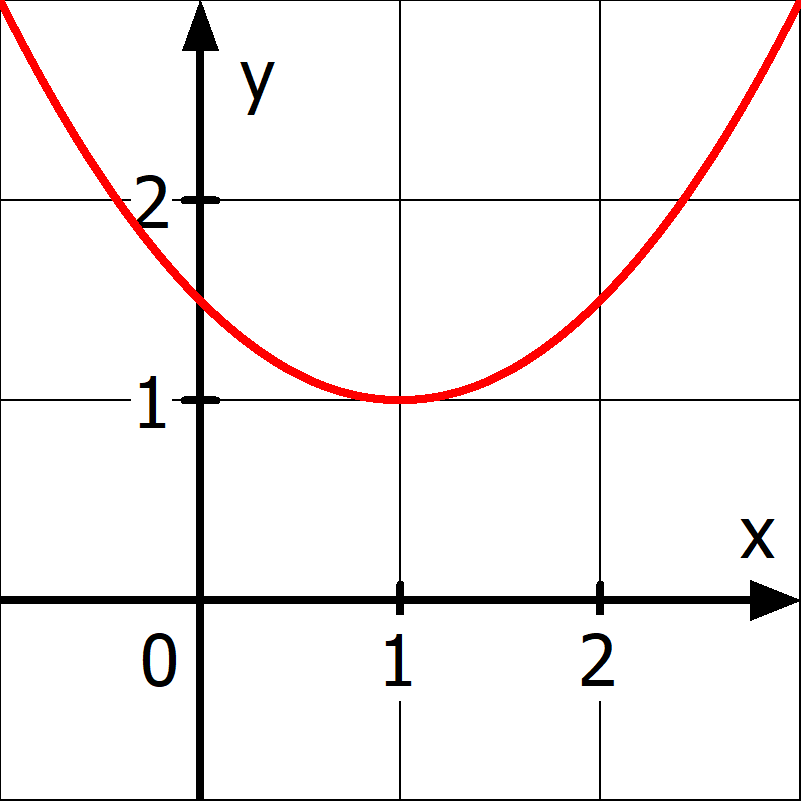
\includegraphics[width=\textwidth]{\ableitung/pics/TPBsp.png}
	\end{minipage}}%
	\adjustbox{valign=t, padding = 0ex 0ex 2ex 0ex}{\begin{minipage}{\textwidth/\real{3}-2ex}
			\centering\includegraphics[width=\textwidth]{\ableitung/pics/TPBspAbl\iftoggle{ausfuellen}{}{_empty}.png}
	\end{minipage}}%
    \adjustbox{valign=t}{\begin{minipage}{\textwidth/\real{3}}
        \textcolor{loes}{Der Tiefpunkt tritt am Übergang von monoton fallend zu monoton wachsend von \(f(x)\) und damit an der NST mit -+VZW der Ableitung auf.}
    \end{minipage}}%
\end{minipage}

\bigskip

\textbf{Sattelpunkt}

Ein Sattelpunkt ist kein Extrempunkt, jedoch ist die Ableitung am Sattelpunkt ebenfalls Null.

\medskip

\begin{minipage}{\textwidth}
    \adjustbox{valign=t, padding = 0ex 0ex 2ex 0ex}{\begin{minipage}{\textwidth/\real{3}-2ex}
			\centering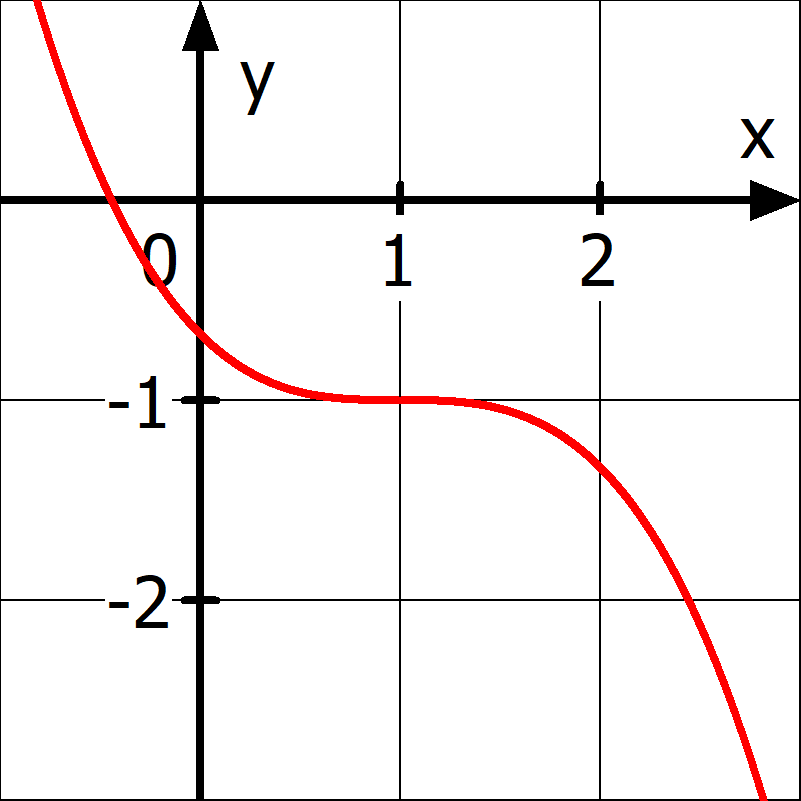
\includegraphics[width=\textwidth]{\ableitung/pics/SPBsp.png}
	\end{minipage}}%
    \adjustbox{valign=t, padding = 0ex 0ex 2ex 0ex}{\begin{minipage}{\textwidth/\real{3}-2ex}
			\centering\includegraphics[width=\textwidth]{\ableitung/pics/SPBspAbl\iftoggle{ausfuellen}{}{_empty}.png}
	\end{minipage}}%
    \adjustbox{valign=t}{\begin{minipage}{\textwidth/\real{3}}
            \textcolor{loes}{Ein Sattelpunkt tritt auf, wenn die Ableitung eine NST ohne VZW hat.}
    \end{minipage}}%
\end{minipage}
\newpage
%%%%%%%%%%%%%%%%%%%%%%%%%%%%%%%%%%%%%%%%%%%%%%%%%%%%%%%%%%%%%%%%%%%%%%%%%%%%%%%%%%%%%%%%%%%%%%%%%%%%%%%
\iftoggle{qrcode}{\setlength{\qrheight}{2.5cm}}{\setlength{\qrheight}{0cm}}%
\newlength{\extremTableWidth}%
\setlength{\extremTableWidth}{\linewidth-\qrheight}%
\begin{minipage}{\textwidth}
    \adjustbox{valign=t, padding =0ex 0ex 0ex 0ex}{\begin{minipage}{\extremTableWidth}
        {\setlength{\tabcolsep}{0pt}%
            \begin{tabular}{p{\extremTableWidth/\real{3}}p{\extremTableWidth/\real{3}}p{\extremTableWidth/\real{3}}}
                Hochpunkt HP&Tiefpunkt TP&Sattelpunkt SP\\
                \midrule
                \multicolumn{3}{c}{\textcolor{loes}{NST in der Ableitung: \(f'(x)=0\)}}\vspace{1cm}\\
                \textcolor{loes}{NST mit +-VZW}&\textcolor{loes}{NST mit -+VZW}&\textcolor{loes}{NST ohne VZW}\\
                \bottomrule
        \end{tabular}}
    \end{minipage}}%
    \iftoggle{qrcode}{\adjustbox{valign=t, padding =0ex 0ex 0ex 0ex}{\begin{minipage}{\qrheight}%
            \href{https://www.geogebra.org/m/ecphwwvv}{
\includegraphics[height=\qrheight]{\ableitung/pics/ExtrempunkteQR.png}}%
        \end{minipage}}}{}%
\end{minipage}%

\bigskip

Eine Möglichkeit auf den VZW der Ableitung zu prüfen ist die zweite Ableitung \(f''(x)\):

Ist \(x_0\) eine NST der ersten Ableitung \(f'(x_0)=0\) so gilt:

\bigskip

\begin{minipage}{\textwidth}
	\adjustbox{valign=t}{\begin{minipage}{0.7\textwidth}
			\(f''(x_0)<0\): \textcolor{loes}{\(f(x)\) hat bei \(x_0\) einen Hochpunkt. Da die zweite Ableitung negativ ist, muss die erste Ableitung bei \(x_0\) fallen, d.h. von oben nach unten verlaufen. Daher hat die erste Ableitung einen +-VZW und \(f(x)\) damit einen Hochpunkt.}
	\end{minipage}}%
	\adjustbox{valign=t, padding = 3ex 0ex 0ex 0ex}{\begin{minipage}{0.3\textwidth-3ex}
			\centering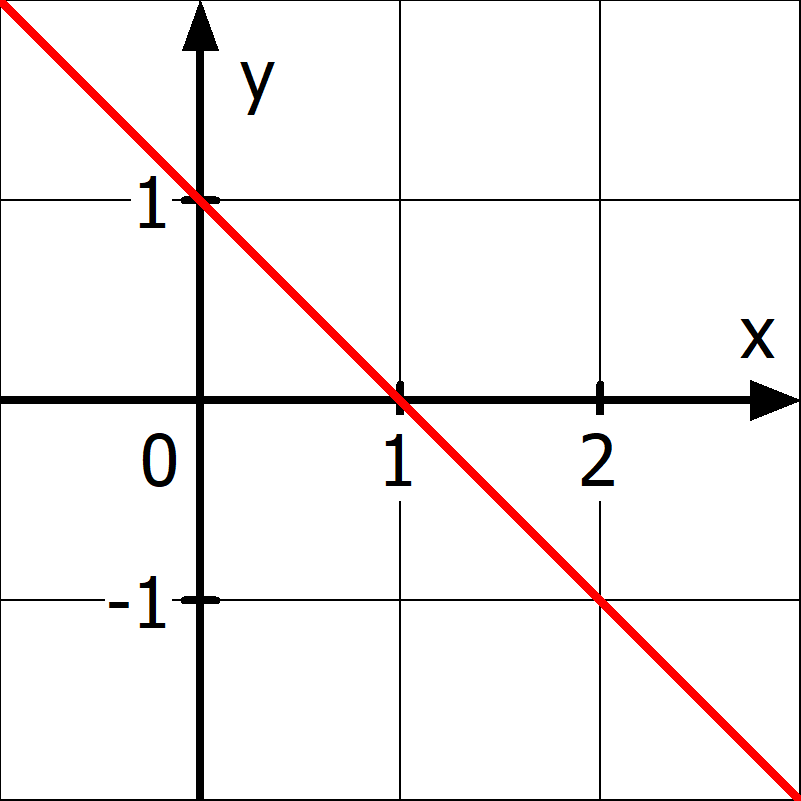
\includegraphics[width=\textwidth]{\ableitung/pics/AblNST2.png}
	\end{minipage}}%
\end{minipage}

\vspace{1.5ex}
\par\noindent\rule{\textwidth}{0.4pt}

\vspace{1.5ex}

\begin{minipage}{\textwidth}
	\adjustbox{valign=t}{\begin{minipage}{0.7\textwidth}
			\(f''(x_0)>0\): \textcolor{loes}{\(f(x)\) hat bei \(x_0\) einen Tiefpunkt. Da die zweite Ableitung positiv ist, muss die erste Ableitung bei \(x_0\) steigen, d.h. von unten nach oben verlaufen. Daher hat die erste Ableitung einen -+VZW und \(f(x)\) damit einen Tiefpunkt.}
	\end{minipage}}%
	\adjustbox{valign=t, padding = 3ex 0ex 0ex 0ex}{\begin{minipage}{0.3\textwidth-3ex}
			\centering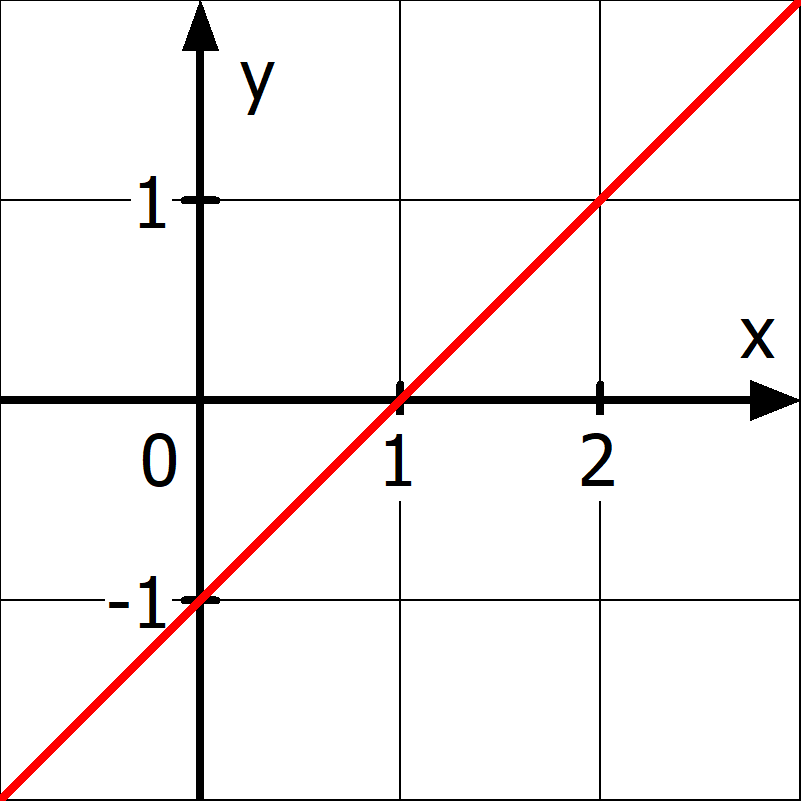
\includegraphics[width=\textwidth]{\ableitung/pics/AblNST1.png}
	\end{minipage}}%
\end{minipage}

\vspace{1.5ex}
\par\noindent\rule{\textwidth}{0.4pt}

\vspace{1.5ex}

\begin{minipage}{\textwidth}
	\adjustbox{valign=t}{\begin{minipage}{0.7\textwidth}
			\(f''(x_0)=0\): \textcolor{loes}{Keine Aussage möglich! \(f(x)\) kann bei \(x_0\) einen HP, TP oder SP haben. Der VZW muss auf andere Art und Weise geprüft werden!}
	\end{minipage}}%
	\adjustbox{valign=t, padding = 3ex 0ex 0ex 0ex}{\begin{minipage}{0.3\textwidth-3ex}
			\centering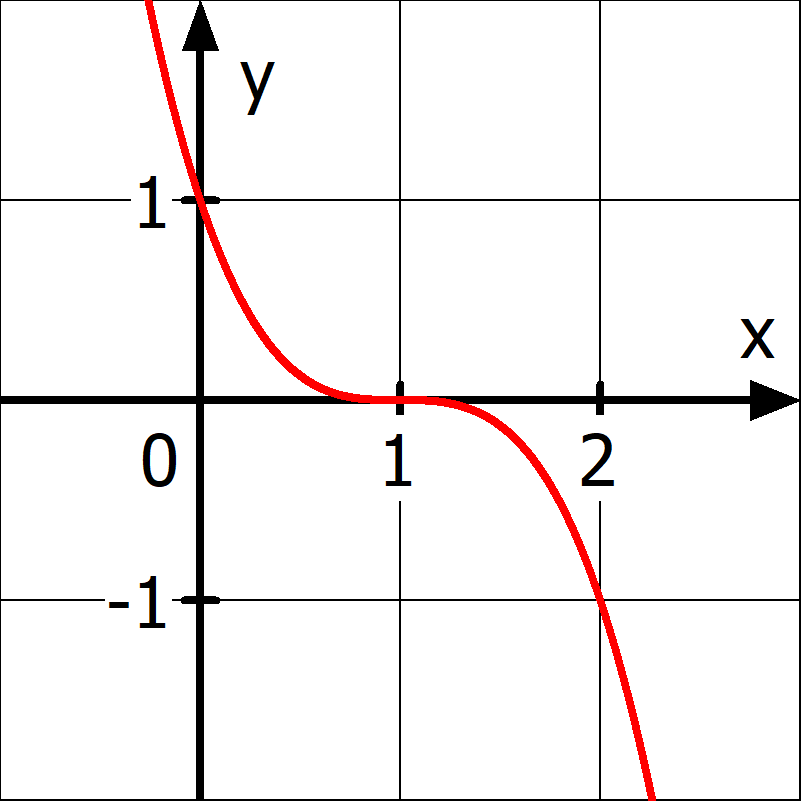
\includegraphics[width=\textwidth]{\ableitung/pics/AblNST4.png}
	\end{minipage}}%
\end{minipage}

\vspace{2.5ex}

\begin{minipage}{\textwidth}
	\adjustbox{valign=t}{\begin{minipage}{0.3\textwidth-3ex}
			\centering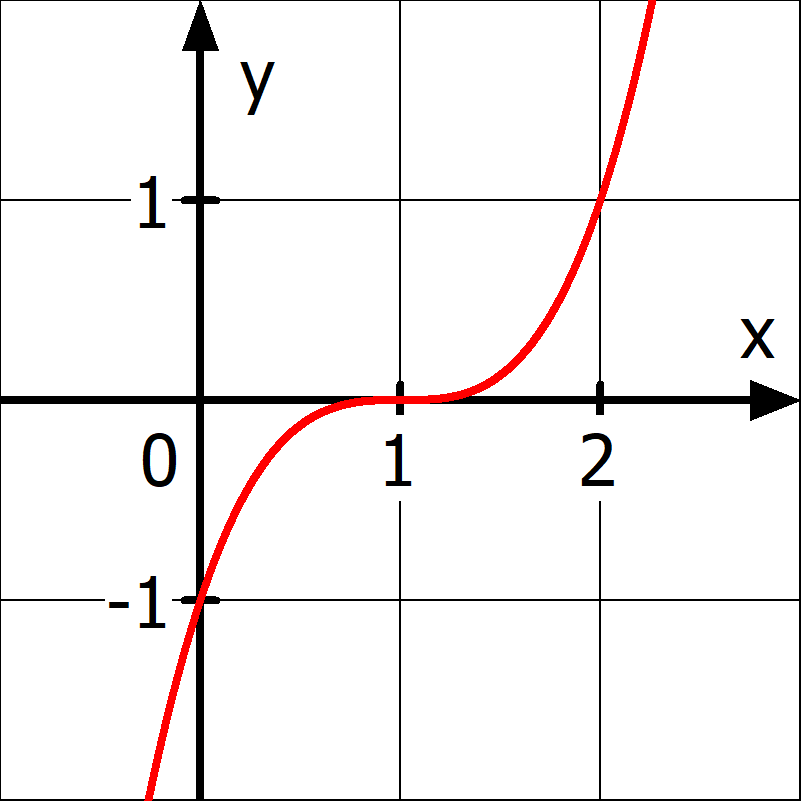
\includegraphics[width=\textwidth]{\ableitung/pics/AblNST3.png}
	\end{minipage}}%
	\adjustbox{valign=t, padding = .05\textwidth+4.5ex 0ex 0ex 0ex}{\begin{minipage}{0.3\textwidth-3ex}
			\centering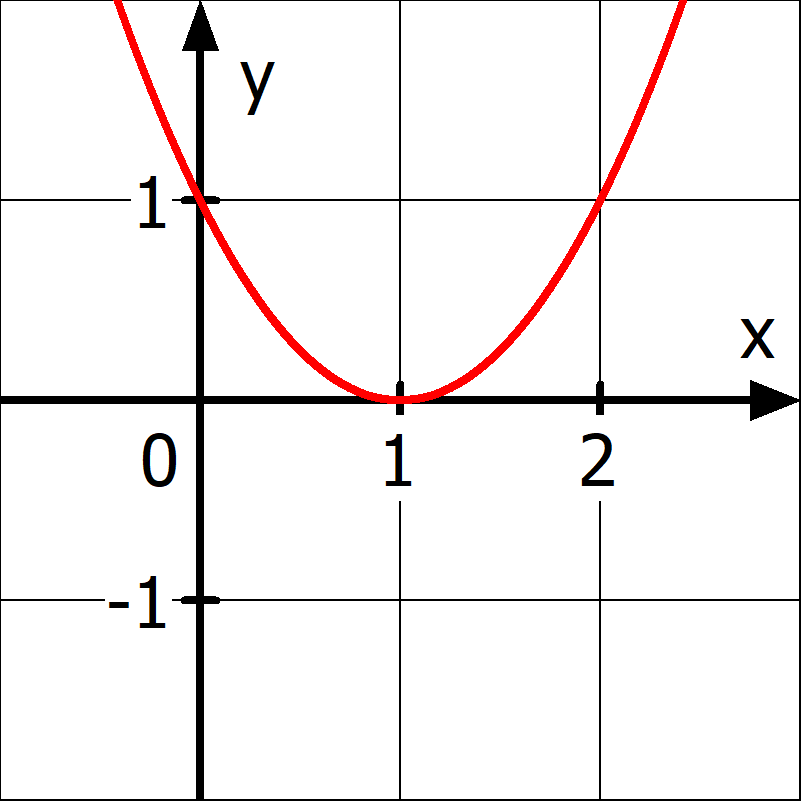
\includegraphics[width=\textwidth]{\ableitung/pics/AblNST5.png}
	\end{minipage}}%
	\adjustbox{valign=t, padding = .05\textwidth+4.5ex 0ex 0ex 0ex}{\begin{minipage}{0.3\textwidth-3ex}
			\centering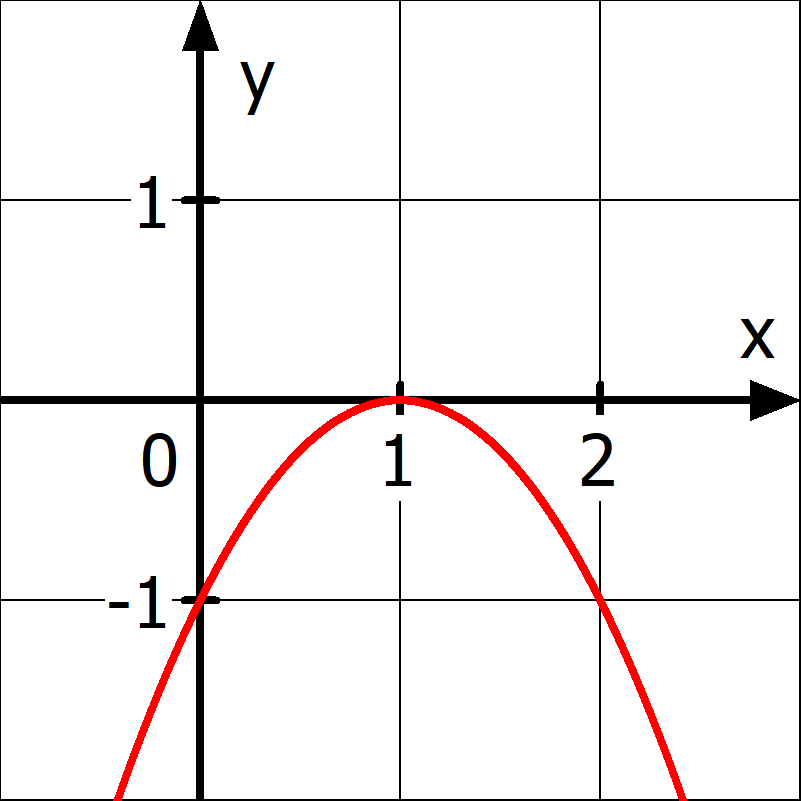
\includegraphics[width=\textwidth]{\ableitung/pics/AblNST6.png}
	\end{minipage}}%
\end{minipage}
\newpage
%%%%%%%%%%%%%%%%%%%%%%%%%%%%%%%%%%%%%%%%%%%%%%%%%%%%%%%%%%%%%%%%%%%%%%%%%%%%%%%%%%%%%%%%%%%%%%%%%%%%%%%
\begin{Exercise}[title={\raggedright Bestimme die Extrem- und Sattelpunkte.}, label=extrempunkteA1]
	\begin{enumerate}[label=\alph*)]
		\item \(f_1(x)=-x^2+2x+1\)
		\item \(f_2(x)=2,5x^2-5x-0,5\)
		\item \(f_3(x)=\frac{1}{3}x^3-x^2-\frac{3}{2}\)
		\item \(f_4(x)=\frac{2}{3}x^3-3x^2+4x\)
		\item \(f_5(x)=-\frac{1}{30}x^3-\frac{1}{10}x^2+\frac{3}{10}x+1\)
		\item \(f_6(x)=-\frac{1}{6}x^3-\frac{3}{2}x^2-\frac{9}{2}x\)
		\item \(f_7(x)=x^3-3x+3\)
		\item \(f_8(x)=2x^3+3x^2-4,4x-3\)
		\item \(f_9(x)=x^3+12x^2+48x+64\)
		\item \(f_{10}(x)=-\frac{1}{24}x^3+2x+2\)
		\item \(f_{11}(x)=\frac{1}{4}x^4+\frac{5}{3}x^3+3x^2\)
		\item \(f_{12}(x)=-1,5x^4-4x^3-4\)
		\item \(f_{13}(x)=\frac{1}{\ln(2)}e^{\ln(2)x}-2x+1\)
		\item \(f_{14}(x)=\frac{1}{20}x^5-\frac{1}{4}x^3-x\)
		\item \(f_{15}(x)=-0,075x^5+1,25x^3-3,375x+1,6\)
		\item \(f_{16}(x)=\frac{32}{7}x^7+7x^4-4x\)
		\item \(f_{17}(x)=\frac{1}{3}e^x-4x\)
		\item \(f_{18}(x)=-\frac{1}{4}e^{-4x}-\frac{1}{2}x+2\)
		\item \(f_{19}(x)=4x^3-18x^2+27x\)
		\item \(f_{20}(x)=2e^{-\frac{1}{2}x}+\frac{5}{2}x-4\)
		\item \(f_{21}(x)=-\frac{4}{3}x^3+6x^2+7x+\frac{1}{6}\)
		\item \(f_{22}(x)=\frac{1}{6}x^6+x\)
		\item \(f_{23}(x)=\frac{1}{15}x^3-\frac{3}{2}x^2+10x+\frac{1}{3}\)
		\item \(f_{24}(x)=8x^3-36x^2+54x-43\)
		\item \(f_{25}(x)=\frac{1}{5}x^5+\frac{4}{3}x^3-5x+\frac{8}{15}\)
		\item \(f_{26}(x)=-4e^{2x}+x+2\)
	\end{enumerate}
\end{Exercise}
%%%%%%%%%%%%%%%%%%%%%%%%%%%%%%%%%%%%%%%%%
\begin{Answer}[ref=extrempunkteA1]
	\begin{enumerate}[label=\alph*)]
		\item \(f_1(x):\ H(1\vert 2)\)
		\item \(f_2(x):\ T(1\vert -3)\)
		\item \(f_3(x):\ H(0\vert -\frac{3}{2}),\ T(2\vert -\frac{17}{6})\)
		\item \(f_4(x):\ H(1\vert \frac{5}{3}),\ T(2\vert \frac{4}{3})\)
		\item \(f_5(x):\ T(-3\vert \frac{1}{10}),\ H(1\vert \frac{7}{6})\)
		\item \(f_6(x):\ S(-3\vert \frac{9}{2})\)
		\item \(f_7(x):\ H(-1\vert 5),\ T(1\vert 1)\)
		\item \(f_8(x):\ H(-1,5\vert 3,75),\ T(0,5\vert -4,25)\)
		\item \(f_9(x):\ S(-4\vert 0)\)
		\item \(f_{10}(x):\ T(-4\vert -\frac{10}{3}),\ H(4\vert \frac{22}{3})\)
		\item \(f_{11}(x):\ T_1(-3\vert \frac{9}{4}),\ H(-2\vert \frac{8}{3}),\ T_2(0\vert 0)\)
		\item \(f_{12}(x):\ H(-2\vert 4),\ S(0\vert -4)\)
		\item \(f_{13}(x):\ T(1\vert \frac{2}{\ln(2)}-1)\)
		\item \(f_{14}(x):\ H(-2\vert \frac{12}{5}),\ T(2\vert -\frac{12}{5})\)
		\item \(f_{15}(x):\ H_1(-1\vert 3,8),\ H_2(3\vert 7),\ T_1(-3 \vert -3,8),\ T_2(1\vert -0,6)\)
		\item \(f_{16}(x):\ H(-1\vert \frac{45}{7}),\ T(\frac{1}{2}\vert -\frac{171}{112})\)
		\item \(f_{17}(x):\ T(\ln(12)\vert 4-4\ln(12))\)
		\item \(f_{18}(x):\ H(\frac{1}{4}\ln(2)\vert \frac{18}{5}-\frac{1}{8}\ln(2)\approx 1,79)\)
		\item \(f_{19}(x):\ S(\frac{3}{2}\vert \frac{27}{2})\)
		\item \(f_{20}(x):\ T\left(-2\ln\left(\frac{5}{2}\right)\vert 1-5\ln(5)+\ln(32)\approx -3,58\right)\)
		\item \(f_{21}(x):\ H\left(\frac{7}{2}\vert 41\right)\)
		\item \(f_{22}(x):\ T(-1\vert-\frac{5}{6})\)
		\item \(f_{23}(x):\ H\left(5\vert\frac{127}{6}\right),\ T(10\vert 17)\)
		\item \(f_{24}(x):\ S\left(\frac{3}{2}\vert -16\right)\)
		\item \(f_{25}(x):\ H(-1\vert 4),\ T(\left(1\vert -\frac{44}{15}\right)\)
		\item \(f_{26}(x):\ H\left(-\frac{3}{2}\ln(2)\vert \frac{3}{2}-\frac{3}{2}\ln(2)\approx 4,89\right)\)
	\end{enumerate}
\end{Answer}